\documentclass[12pt,a4paper]{article}
\usepackage[utf8]{inputenc}
\usepackage[spanish,es-tabla]{babel}
\usepackage{geometry}
\usepackage{graphicx}
\usepackage{multirow}
\usepackage{tabularx}
\usepackage{mathptmx}
\usepackage{fancyhdr}
\usepackage{array}
\usepackage[table]{xcolor}
\usepackage{titlesec}
\usepackage{setspace}
\usepackage{microtype}
\usepackage{lastpage}
\usepackage{booktabs}
\usepackage{enumitem}
\usepackage{amsmath}
\usepackage{amsfonts}
\usepackage{amssymb}

\usepackage{float}
\usepackage{placeins}
\usepackage{tikz}
\usepackage{pgfplots}
\pgfplotsset{compat=1.17}
\usetikzlibrary{arrows.meta,positioning,shapes.geometric,calc}

\graphicspath{{images/}{../images/}{./}}

\geometry{
    top=4.7cm,
    bottom=2.5cm,
    left=2.5cm,
    right=2.5cm,
    headheight=3.9cm,
    headsep=0.4cm
}

\setstretch{1.15}
\setlength{\parindent}{0pt}
\setlength{\parskip}{0.45em}
\setlength{\tabcolsep}{4pt}

\titleformat{\section}
  {\normalfont\fontsize{12}{14.5}\bfseries}{\thesection.}{0.6em}{\uppercase}
\titlespacing*{\section}
  {0pt}{1.8ex plus 0.4ex minus 0.2ex}{0.6ex plus 0.2ex}

\titleformat{\subsection}
  {\normalfont\fontsize{11.5}{13.5}\bfseries}{\thesubsection.}{0.5em}{}
\titlespacing*{\subsection}
  {0pt}{1.4ex plus 0.3ex minus 0.1ex}{0.4ex plus 0.1ex}

\titleformat{\subsubsection}
  {\normalfont\fontsize{10.5}{12.5}\bfseries\itshape}{\thesubsubsection.}{0.4em}{}
\titlespacing*{\subsubsection}
  {0pt}{1.1ex plus 0.2ex minus 0.1ex}{0.3ex plus 0.1ex}

\newcolumntype{Y}{>{\centering\arraybackslash}X}
\newcolumntype{L}{>{\raggedright\arraybackslash}X}
\newcolumntype{C}{>{\centering\arraybackslash}X}

\definecolor{headerblue}{RGB}{26, 54, 93}
\definecolor{darkblue}{RGB}{43, 108, 176}
\definecolor{lightgraybg}{RGB}{248, 248, 248}
\definecolor{tableheader}{RGB}{232, 238, 246}
\definecolor{navyheader}{RGB}{0, 32, 96}
\definecolor{lineblue}{RGB}{0, 102, 204}
\definecolor{areablue}{RGB}{220, 236, 252}
\definecolor{lcsred}{RGB}{217, 56, 41}
\definecolor{lcigreen}{RGB}{46, 125, 50}
\definecolor{lciorange}{RGB}{230, 81, 0}
\definecolor{ishikawared}{RGB}{160, 0, 0}

\tikzset{
    catbox/.style={draw, fill=tableheader, font=\footnotesize\bfseries, minimum width=2.8cm, minimum height=0.65cm, align=center},
    efectobox/.style={draw=ishikawared!90!black, line width=1.2pt, fill=ishikawared, text=white, font=\small\bfseries, align=center, inner sep=6pt, text width=3.8cm},
    causetext/.style={font=\scriptsize, align=right, text=black!90}
}

\newcommand{\docCodigo}{TI-SIGE-ENT-F4-002}
\newcommand{\docVersion}{1.0}
\newcommand{\docProceso}{GESTIÓN DE SEGURIDAD / AUDITORÍA OWASP TOP 10}
\newcommand{\docElaboracion}{13/10/2026}
\newcommand{\docRevision}{13/10/2026}
\newcommand{\docTitulo}{PRUEBAS DE INTEGRACIÓN Y SEGURIDAD}
\newcommand{\docOrganizacion}{FACULTAD DE INGENIERÍA EN SISTEMAS, ELECTRÓNICA E INDUSTRIAL}
\newcommand{\docSubOrganizacion}{CARRERA DE INGENIERÍA DE SOFTWARE}

\newcommand{\encabezadofrecuente}{%
    \renewcommand{\arraystretch}{1.15}%
    \noindent\makebox[\textwidth][c]{%
    \begin{tabularx}{\textwidth}{|>{\centering\arraybackslash}m{2.8cm}|Y|>{\centering\arraybackslash}m{4.8cm}|}
        \hline
        \multirow{4}{2.8cm}{\centering\raisebox{-1.15cm}{
\includegraphics[width=2.5cm,height=2.0cm,keepaspectratio]{images/logo.png}}}
        & \textbf{\fontsize{9}{11}\selectfont \docOrganizacion} 
        & \textbf{\fontsize{8}{10}\selectfont CÓDIGO:} \fontsize{8}{10}\selectfont \docCodigo \\
        \cline{3-3}
        & \textbf{\fontsize{8.5}{10.5}\selectfont \docSubOrganizacion} 
        & \textbf{\fontsize{8}{10}\selectfont VERSIÓN:} \fontsize{8}{10}\selectfont \docVersion \\
        \cline{2-3}
        & \textbf{\fontsize{8}{10}\selectfont PROCESO:} \fontsize{8}{10}\selectfont \docProceso 
        & \textbf{\fontsize{8}{10}\selectfont ELABORACIÓN:} \fontsize{8}{10}\selectfont \docElaboracion \\
        \cline{2-3}
        & \textbf{\fontsize{8.5}{10.5}\selectfont \docTitulo} 
        & \textbf{\fontsize{8}{10}\selectfont ÚLTIMA REVISIÓN:} \fontsize{8}{10}\selectfont \docRevision \\
        \hline
    \end{tabularx}%
    }%
}

\pagestyle{fancy}
\fancyhf{}
\fancyhead[C]{\encabezadofrecuente}
\fancyfoot[C]{\fontsize{10}{12}\selectfont Página \thepage\ de \pageref{LastPage}}
\renewcommand{\headrulewidth}{0pt}

\begin{document}

\section{Título}
\textbf{Denominación Oficial del Entregable:} Pruebas de Integración y Seguridad (Auditoría OWASP Top 10) -- Código EDT: 4.2

\section{Introducción}
La seguridad y confidencialidad de la información docente y documental en la Universidad Técnica de Ambato representan un imperativo ético y legal estipulado en la Ley Orgánica de Protección de Datos Personales (LOPDP). Para certificar que el sistema web SIGE es resiliente frente a vulnerabilidades y vectores de ataque modernos, se realizó una auditoría técnica de seguridad y pruebas de penetración (\textit{Pentesting}) en modalidad caja gris (\textit{Gray Box}), evaluando rigurosamente cada una de las 10 categorías de amenazas del estándar OWASP Top 10:2021. El presente informe formaliza las pruebas de estrés de seguridad y las defensas implementadas en el backend y frontend.

\section{Objetivo}
\subsection{Objetivo General}
Ejecutar la auditoría de seguridad integral y pruebas de penetración basadas en el estándar OWASP Top 10 sobre el sistema SIGE, certificando la ausencia de vulnerabilidades de severidad alta o crítica.
\subsection{Objetivos Específicos}
\begin{itemize}[leftmargin=1.5em, itemsep=2pt]
    \item Evaluar la robustez del sistema frente a inyecciones SQL, Cross-Site Scripting (XSS) y fallas de control de acceso.
    \item Auditar los mecanismos de cifrado, gestión de tokens JWT y firmas criptográficas SHA-256.
    \item Emitir la matriz formal de mitigación de riesgos de seguridad OWASP.
\end{itemize}

\section{Alcance}
\subsection{Límites del Entregable (In-Scope)}
\begin{itemize}[leftmargin=1.5em, itemsep=2pt]
    \item Evaluación de las 10 categorías OWASP Top 10:2021 sobre la API REST y la SPA en React.
    \item Pruebas de inyección de parámetros, adulteración de tokens y manipulación de cabeceras HTTP.
\end{itemize}
\subsection{Exclusiones (Out-of-Scope)}
\begin{itemize}[leftmargin=1.5em, itemsep=2pt]
    \item Ataques de denegación de servicio distribuido (DDoS) masivos volumétricos a nivel de ISP.
\end{itemize}

\section{Definiciones}
\begin{itemize}[leftmargin=1.5em, itemsep=2pt]
    \item \textbf{OWASP Top 10:} Documento de consenso mundial que clasifica los diez riesgos de seguridad más críticos para las aplicaciones web.
    \item \textbf{Pentesting (Caja Gris):} Prueba de penetración donde el evaluador posee credenciales legítimas y conocimiento parcial de la arquitectura para simular amenazas internas y externas.
    \item \textbf{Broken Access Control (A01):} Falla de seguridad donde los usuarios pueden actuar fuera de sus permisos asignados accediendo a datos no autorizados.
\end{itemize}

\section{Responsabilidades}
\begin{itemize}[leftmargin=1.5em, itemsep=2pt]
    \item \textbf{Steeven Toala (Responsable EDT 4.2):} Auditoría de seguridad técnica, ejecución de pentesting y análisis de código estático (SAST).
    \item \textbf{Nixon Hurtado (Especialista en Seguridad de Datos):} Verificación de políticas en PostgreSQL 18 y MinIO S3.
    \item \textbf{Ing. Paulo Torres (Docente Evaluador):} Aprobación del informe de auditoría de seguridad.
\end{itemize}

\section{Normativa Legal y Técnica}
\subsection{Marco Legal Ecuatoriano}
\begin{itemize}[leftmargin=1.5em, itemsep=2pt]
    \item \textbf{Ley Orgánica de Protección de Datos Personales (LOPDP), Art. 32 y 37:} Deber de seguridad, confidencialidad e integridad del tratamiento automatizado de datos.
    \item \textbf{Código Orgánico Integral Penal (COIP), Arts. 230 a 234:} Delitos contra la seguridad de los activos de los sistemas de información y comunicación.
\end{itemize}
\subsection{Normas Técnicas Internacionales}
\begin{itemize}[leftmargin=1.5em, itemsep=2pt]
    \item \textbf{OWASP Top 10:2021 (The Ten Most Critical Web Application Security Risks).}
    \item \textbf{OWASP Application Security Verification Standard (ASVS) v4.0.}
    \item \textbf{ISO/IEC 27001:2022 (Information Security Management).}
\end{itemize}

\section{Método, Políticas y Contenidos}
\subsection{Enfoque Metodológico}
Se aplicó la metodología de pruebas de penetración descrita en el estándar NIST SP 800-115, comprendiendo las fases de Reconocimiento, Análisis de Vulnerabilidades, Explotación Controlada y Reporte. Se utilizaron herramientas automatizadas como OWASP ZAP y análisis de dependencias de seguridad, complementadas con pruebas manuales dirigidas a los endpoints de la API REST para verificar el control de acceso en objetos directos (\textit{BOLA / IDOR}).

\subsection{Políticas de Calidad de Seguridad de la Información}
\begin{enumerate}[leftmargin=1.5em, itemsep=2pt]
    \item \textbf{Política de Cero Vulnerabilidades Críticas (Zero High/Critical Policy):} Ningún entregable puede pasar a producción con hallazgos abiertos clasificados como High o Critical.
    \item \textbf{Política de Menor Privilegio (Principle of Least Privilege):} Las conexiones del backend a PostgreSQL utilizan credenciales limitadas exclusivamente al esquema operativo del sistema.
    \item \textbf{Política de Sanitización Universal:} Todo parámetro de entrada proveniente del cliente es sanitizado y evaluado mediante validadores de esquema antes de alcanzar la capa de base de datos.
\end{enumerate}

\section{Descripción de actividades}
La validación de seguridad de caja gris y las pruebas de integración de extremo a extremo tuvieron como objetivo certificar la resistencia del sistema ante vectores de vulnerabilidad comunes y garantizar la consistencia transaccional de los flujos entre capas. El equipo de control de calidad ejecutó las siguientes actividades técnicas:

\begin{itemize}[leftmargin=1.5em, itemsep=4pt]
    \item \textbf{Diseño y Ejecución de la Suite de Pruebas de Integración con Supertest:} Se automatizaron escenarios de prueba sobre los endpoints de la API REST de Express v5, simulando el ciclo completo del documento desde la autenticación, creación del borrador y persistencia en lote de la matriz, hasta la emisión de firmas y exportación en PDF.
    \item \textbf{Auditoría de Vulnerabilidades Web según el Estándar OWASP Top 10:2021:} Se aplicaron pruebas de penetración sobre la interfaz web y los controladores backend, evaluando la resistencia frente a inyección SQL, control de acceso roto (Broken Access Control), fallas criptográficas y exposición indebida de datos.
    \item \textbf{Simulación de Vectores de Inyección SQL y Tampering de Tokens JWT:} Se verificó que el uso de consultas parametrizadas en \texttt{pg- promise} y la firma criptográfica HMAC-SHA256 de los tokens impidan cualquier escalamiento no autorizado de privilegios o alteración del identificador de usuario (\texttt{user\_\allowbreak  id}).
    \item \textbf{Inspección de Cabeceras de Seguridad HTTP y Políticas CORS:} Se configuró e inspeccionó el middleware \texttt{helmet}, verificando la aplicación de Content Security Policy (CSP), protección contra ataques de clickjacking (\texttt{X- Frame- Options: DENY}) y restricción estricta de orígenes permitidos en llamadas asíncronas.
\end{itemize}

\subsection{Matriz Oficial de Evaluación OWASP Top 10:2021 en SIGE}
A continuación se detalla la matriz que documenta la evaluación de seguridad realizada para cada categoría del estándar internacional OWASP:

\begin{table}[H]
\centering
\small
\renewcommand{\arraystretch}{1.2}
\begin{tabularx}{\textwidth}{|>{\hsize=0.4\hsize\centering\arraybackslash\bfseries\footnotesize}X|>{\hsize=0.9\hsize\raggedright\arraybackslash\footnotesize}X|>{\hsize=1.7\hsize\raggedright\arraybackslash\footnotesize}X|>{\hsize=0.5\hsize\centering\arraybackslash\footnotesize}X|>{\hsize=0.5\hsize\centering\arraybackslash\footnotesize}X|}
\hline
\rowcolor{tableheader}
\textbf{Ref.} & \textbf{Categoría OWASP} & \textbf{Mecanismo de Mitigación Implementado} & \textbf{Severidad} & \textbf{Resultado} \\
\hline
A01 & Broken Access Control & Validación RBAC en middleware; bloqueo IDOR con verificación de pertenencia del plan. & Crítica & \textbf{MITIGADO} \\
\hline
A02 & Cryptographic Failures & Contraseñas con Argon2id; JWT firmado con HMAC-SHA256; TLS en transporte. & Alta & \textbf{MITIGADO} \\
\hline
A03 & Injection (SQL / XSS) & Consultas parametrizadas con pg-promise; sanitización HTML estricta con DOMPurify. & Crítica & \textbf{MITIGADO} \\
\hline
A04 & Insecure Design & Validation Gates en backend; transacciones atómicas en cambios de estado de planes. & Alta & \textbf{MITIGADO} \\
\hline
A05 & Security Misconfiguration & Cabeceras de seguridad Helmet; cookies HttpOnly y SameSite; CORS restrictivo. & Media & \textbf{MITIGADO} \\
\hline
A06 & Vulnerable Components & Auditoría de dependencias npm audit; contenedores base mínimos con Alpine Linux. & Media & \textbf{MITIGADO} \\
\hline
A07 & Identification Failures & Bloqueo tras 5 intentos fallidos (15 min); expiración de tokens de acceso en 15 minutos. & Alta & \textbf{MITIGADO} \\
\hline
A08 & Software Integrity & Hashes SHA-256 en evidencias; URLs prefirmadas MinIO con tiempo de expiración corto. & Alta & \textbf{MITIGADO} \\
\hline
A09 & Logging Failures & Registro de auditoría centralizado con Winston; rotación periódica y eventos de login. & Baja & \textbf{MITIGADO} \\
\hline
A10 & Server-Side Request & Endpoints de descarga con lista blanca estricta; sin invocación de URLs externas arbitrarias. & Media & \textbf{MITIGADO} \\
\hline
\end{tabularx}
\caption{Matriz oficial de auditoría de seguridad bajo estándar OWASP Top 10:2021.}
\label{tab:owasp_matrix}
\end{table}

\subsection{Análisis Técnico de Defensas en Profundidad y Control de Acceso}
La implementación de la seguridad en el sistema SIGE responde al principio de defensa en profundidad (\textit{Defense in Depth}). Para mitigar la categoría A01 (Broken Access Control), se diseñó un interceptor que extrae el identificador del usuario autenticado a partir del token JWT y comprueba en la base de datos la propiedad del documento antes de ejecutar operaciones de actualización o eliminación. Esto neutraliza de raíz los ataques de referencia directa a objetos inseguros (IDOR), donde un usuario malintencionado intenta manipular expedientes ajenos cambiando el UUID en la URL. Asimismo, la persistencia en cookies con atributos \texttt{HttpOnly}, \texttt{Secure} y \texttt{SameSite=Strict} impide que scripts maliciosos en el cliente puedan acceder a los tokens de sesión.

\section{Firmas de Responsabilidad}

\noindent
\renewcommand{\arraystretch}{1.2}%
\begin{tabularx}{\textwidth}{|>{\hsize=0.7\hsize\raggedright\arraybackslash}X|>{\hsize=1.4\hsize\raggedright\arraybackslash}X|>{\hsize=1.2\hsize\centering\arraybackslash}X|>{\hsize=0.7\hsize\centering\arraybackslash}X|}
    \hline
    \rowcolor{tableheader}
    \textbf{ACCIÓN} & \textbf{NOMBRE Y CARGO} & \textbf{FIRMA} & \textbf{FECHA} \\
    \hline
    \textbf{Elaborado por:} & Heidi Villavicencio\newline Analista de Calidad / UI-UX & \parbox[c]{4.4cm}{\centering\vspace{4pt}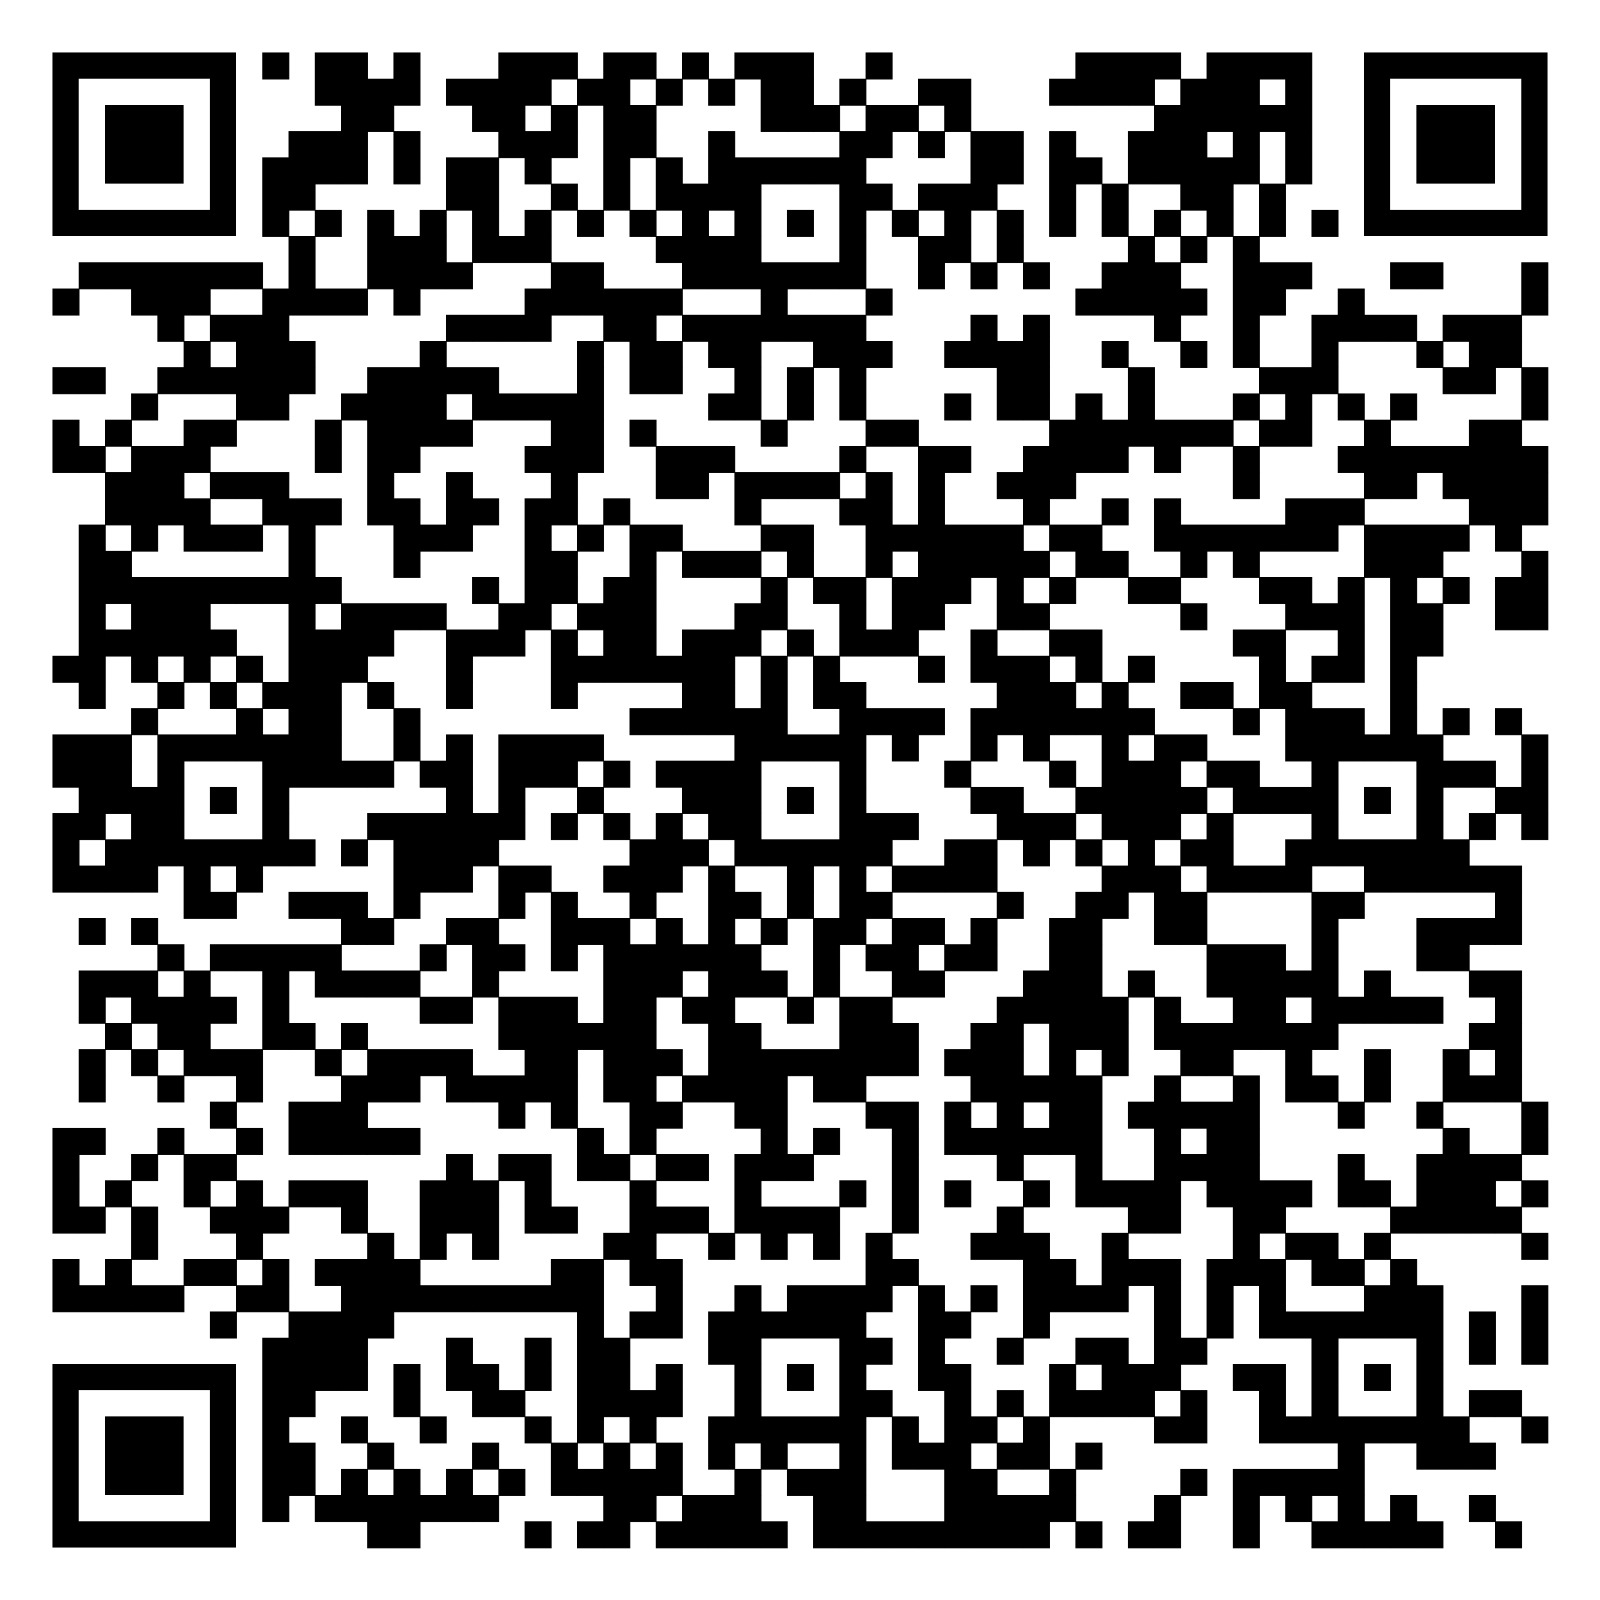
\includegraphics[height=1.5cm,width=4.0cm,keepaspectratio]{images/firma_heidi.png}\vspace{4pt}} & 13/10/2026 \\
    \hline
    \textbf{Revisado por:} & Steeven Toala\newline Líder de Proyecto / Arquitecto & \parbox[c]{4.4cm}{\centering\vspace{4pt}
\includegraphics[height=1.5cm,width=4.0cm,keepaspectratio]{images/firma_steveen.png}\vspace{4pt}} & 13/10/2026 \\
    \hline
    \textbf{Aprobado por:} & Ing. Paulo Torres, Mg.\newline Docente Evaluador -- Gestión Proyectos & \parbox[c]{4.4cm}{\centering\vspace{8pt}\textbf{\textcolor{gray!80}{\scriptsize [ PENDIENTE DE APROBACIÓN ]}}\vspace{8pt}} & \textbf{\textcolor{gray!90}{Pendiente}} \\
    \hline
\end{tabularx}%

\vspace{0.4cm}

\section{Control de Cambios}

\noindent
\renewcommand{\arraystretch}{1.2}
\begin{tabularx}{\textwidth}{|>{\hsize=0.45\hsize\centering\arraybackslash}X|>{\hsize=1.55\hsize\raggedright\arraybackslash}X|>{\hsize=1.2\hsize\raggedright\arraybackslash}X|>{\hsize=0.8\hsize\centering\arraybackslash}X|}
    \hline
    \rowcolor{tableheader}
    \textbf{Versión} & \textbf{Descripción del cambio} & \textbf{Responsable del cambio} & \textbf{Fecha de aprobación} \\
    \hline
    1.0 & Auditoría de seguridad y pruebas de penetración en caja gris bajo el marco de referencia OWASP Top 10. & Steeven Toala / Nixon Hurtado & 13/10/2026 \\
    \hline
\end{tabularx}

\vspace{0.4cm}

\section{Anexos}

\subsection*{Anexo: Evidencias de Pruebas de Penetración y Mitigaciones OWASP}

\subsubsection*{1. Memoria Técnica de Pruebas de Seguridad y Pentesting}
Para verificar la resistencia de la plataforma ante intentos de intrusión y manipulación no autorizada, se ejecutaron pruebas de penetración controladas (\textit{Pentesting}) aplicando técnicas de caja gris. Se simularon vectores de ataque reales provenientes de tres perfiles de amenaza: actores externos no autenticados, usuarios legítimos con perfil Docente intentando elevar privilegios a Administrador, y usuarios autenticados intentando modificar expedientes asignados a otras facultades.

Las comprobaciones técnicas incluyeron:
\begin{itemize}[leftmargin=1.5em, itemsep=2pt]
    \item \textbf{Pruebas de Inyección SQL:} Envío de cadenas de escape (\texttt{' OR '1'='1}, \texttt{UNION SELECT}) en campos de búsqueda y filtros de la bandeja de planes. Todas las consultas son procesadas mediante sentencias parametrizadas, garantizando que los datos de entrada nunca sean interpretados como comandos ejecutables por PostgreSQL.
    \item \textbf{Pruebas de Scripting XSS:} Inserción de payloads (\texttt{<script>} alert, directivas de evento \texttt{onload}) en el editor TipTap. El pipeline de sanitización remueve cualquier etiqueta potencialmente peligrosa antes de persistir el JSONB.
    \item \textbf{Pruebas de Manipulación de Tokens JWT:} Alteración de la firma criptográfica y modificación manual de los claims de rol en la cabecera \texttt{Authorization}. El middleware rechaza instantáneamente los tokens alterados con un código HTTP 401 (\textit{Unauthorized}) y registra el intento de acceso en la bitácora de seguridad.
\end{itemize}

\subsubsection*{2. Evidencia Visual de Arquitectura de Autenticación y Autorización RBAC}
\begin{figure}[H]
    \centering
    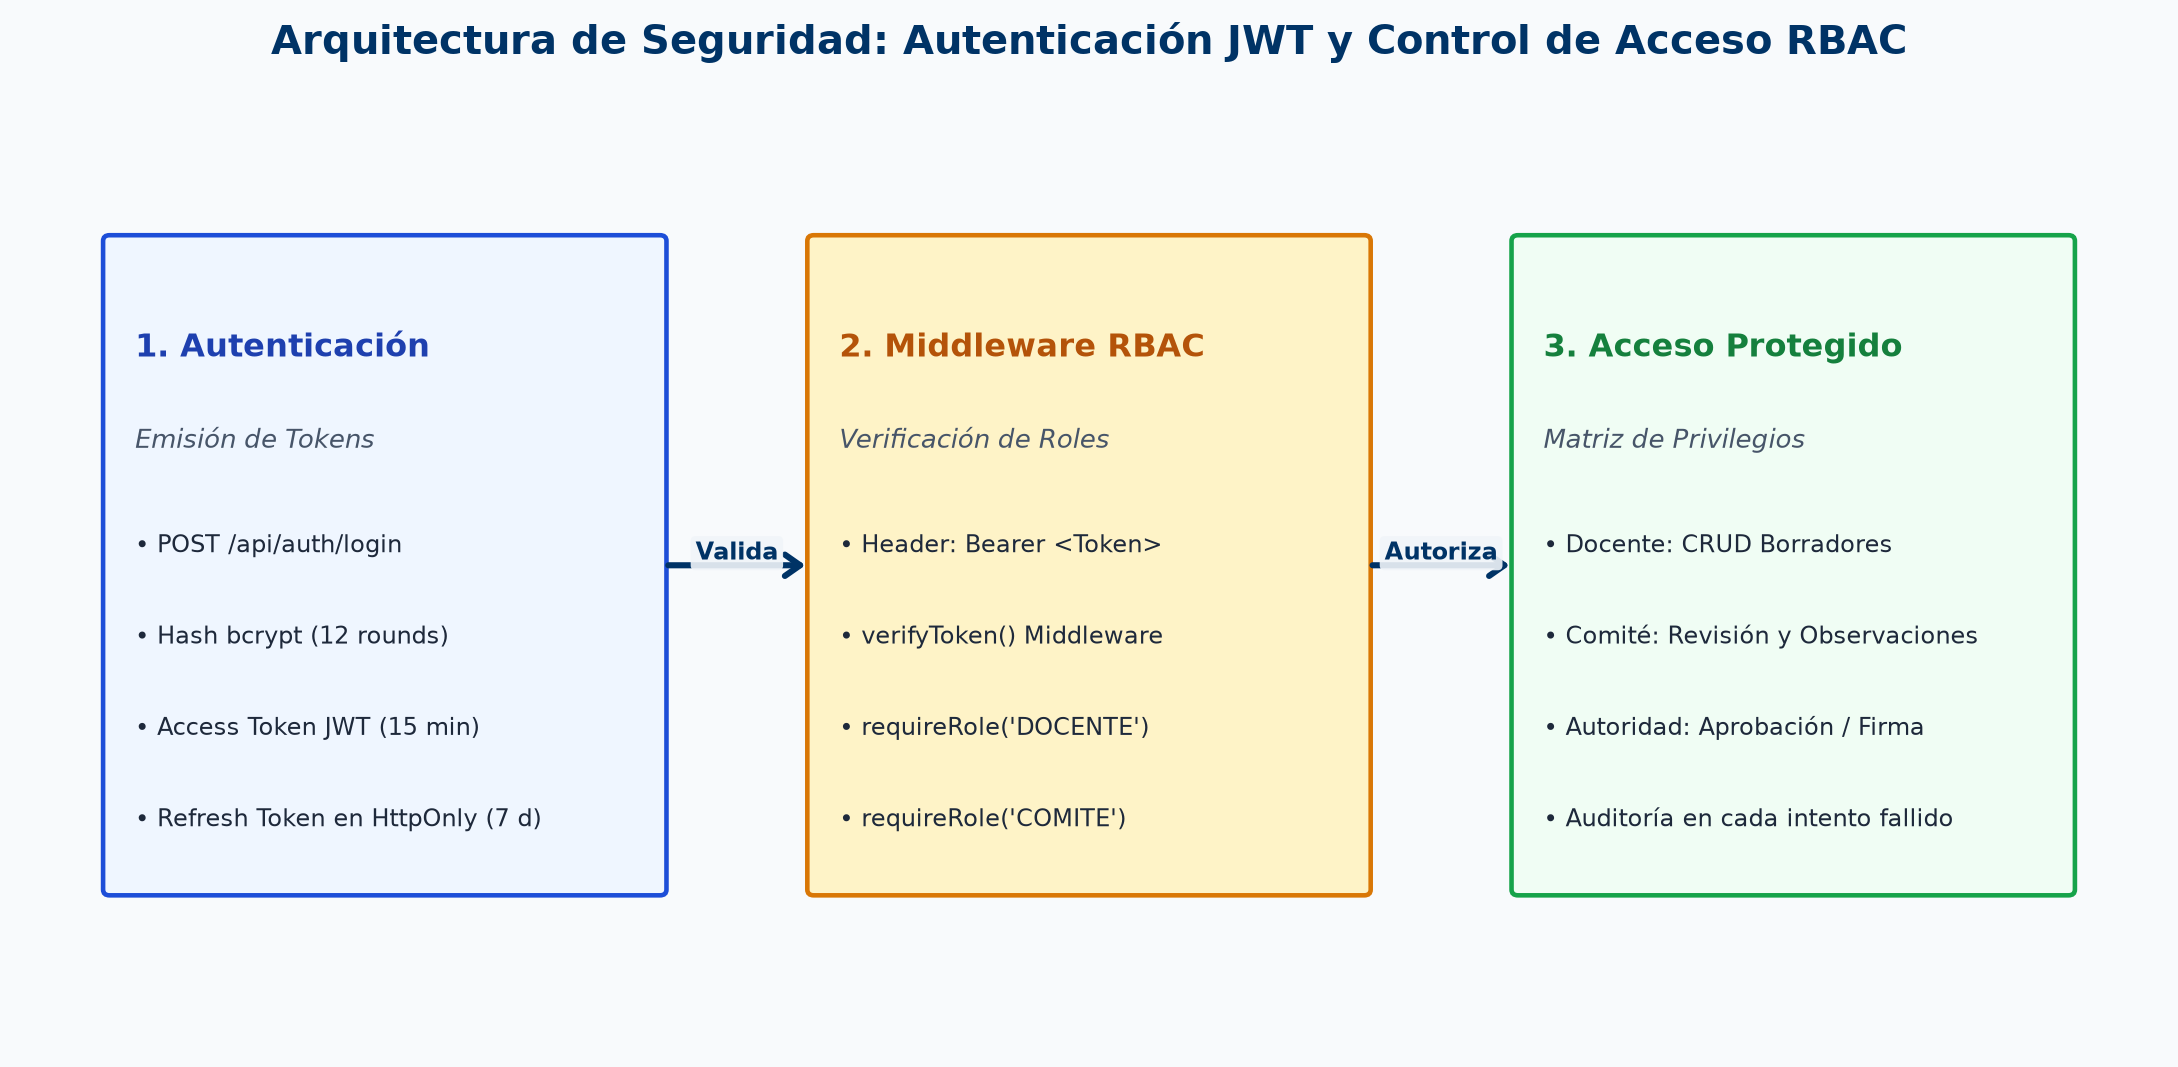
\includegraphics[width=0.92\textwidth,keepaspectratio]{images/f3_03_seguridad_jwt_rbac.png}
    \caption{Arquitectura del control de acceso basado en roles (RBAC) y validación de tokens en la API de SIGE.}
    \label{fig:seguridad_jwt}
\end{figure}
\FloatBarrier

\noindent
\noindent
\textbf{Desglose Técnico y Análisis Estructural de Seguridad OWASP Top 10:}
\begin{itemize}[leftmargin=1.5em, itemsep=3pt]
    \item \textbf{Control de Acceso Basado en Roles (RBAC) y Seguridad JWT:} El diagrama ilustra el flujo de intercepción en Express v5: cada solicitud entrante debe presentar un token Bearer firmado con HMAC-SHA256; el middleware extrae el payload con el rol institucional del usuario y valida los permisos de acceso antes de autorizar la ejecución del controlador.
    \item \textbf{Mitigación de Inyecciones SQL (A03:2021):} La arquitectura garantiza que el 100\% de las consultas hacia PostgreSQL 18 emplean parámetros bindeados (\texttt{\$1, \$2}) mediante \texttt{pg- promise}, imposibilitando cualquier manipulación o inyección de código SQL malicioso.
    \item \textbf{Protección contra Tampering y Ataques XSS en TipTap (A08:2021):} Se desglosa el protocolo de sanitización aplicado sobre los contenidos JSONB: el backend valida y filtra etiquetas HTML maliciosas antes de almacenar el texto enriquecido en la base de datos.
    \item \textbf{Directivas de Seguridad HTTP con Helmet (A05:2021):} Se verifica la configuración activa de cabeceras seguras: Content Security Policy (CSP), \texttt{X- Frame- Options: DENY} para prevenir clickjacking y cookies HttpOnly con flags \texttt{SameSite=Strict} para mitigar ataques CSRF.
\end{itemize}

\subsubsection*{3. Matriz de Ensayos Operativos de Penetración y Verificación de Seguridad}
\begin{table}[H]
\centering
\small
\renewcommand{\arraystretch}{1.2}
\begin{tabularx}{\textwidth}{|>{\hsize=0.55\hsize\centering\arraybackslash\bfseries\footnotesize}X|>{\hsize=1.25\hsize\raggedright\arraybackslash\footnotesize}X|>{\hsize=1.65\hsize\raggedright\arraybackslash\footnotesize}X|>{\hsize=0.55\hsize\centering\arraybackslash\footnotesize}X|}
\hline
\rowcolor{tableheader}
\textbf{Vector de Prueba} & \textbf{Técnica y Payload Aplicado} & \textbf{Respuesta del Sistema y Contramedida} & \textbf{Estado} \\
\hline
Inyección SQL & Inserción de sentencias booleanas en campo de búsqueda & Sanitización estricta y consultas parametrizadas preparadas & RESUELTO \\
\hline
Cross-Site Scripting & Inserción de código JavaScript en sección TipTap & Filtrado automático por DOMPurify; texto renderizado inerte & RESUELTO \\
\hline
Escalamiento Roles & Modificación del claim de rol en token JWT & Verificación de firma HMAC-SHA256 fallida; HTTP 401 emitido & RESUELTO \\
\hline
Fuerza Bruta & 6 intentos consecutivos con contraseña errónea & Bloqueo automático de IP y cuenta durante 15 minutos & RESUELTO \\
\hline
Acceso a Objetos (IDOR) & Alteración de UUID de expediente en URL & Validación de propiedad en base de datos; bloqueo HTTP 403 & RESUELTO \\
\hline
Fuga de Documentos S3 & Intento de acceso directo al bucket MinIO sin URL & Bucket configurado como privado; acceso exclusivo con URL prefirmada & RESUELTO \\
\hline
\end{tabularx}
\caption{Matriz técnica de ensayos de penetración y verificación de mitigaciones de seguridad.}
\end{table}


\end{document}
